\documentclass[aspectratio=3219]{beamer}

\usepackage{graphicx} % Required for inserting images
\usepackage[english,greek]{babel}
\usepackage[utf8x]{inputenc}
\usepackage{xcolor}
\usepackage{tikz}
\usepackage[absolute,overlay]{textpos}

\graphicspath{images/}

\newcommand{\lt}{\latintext}
\newcommand{\gt}{\greektext}

\usebackgroundtemplate{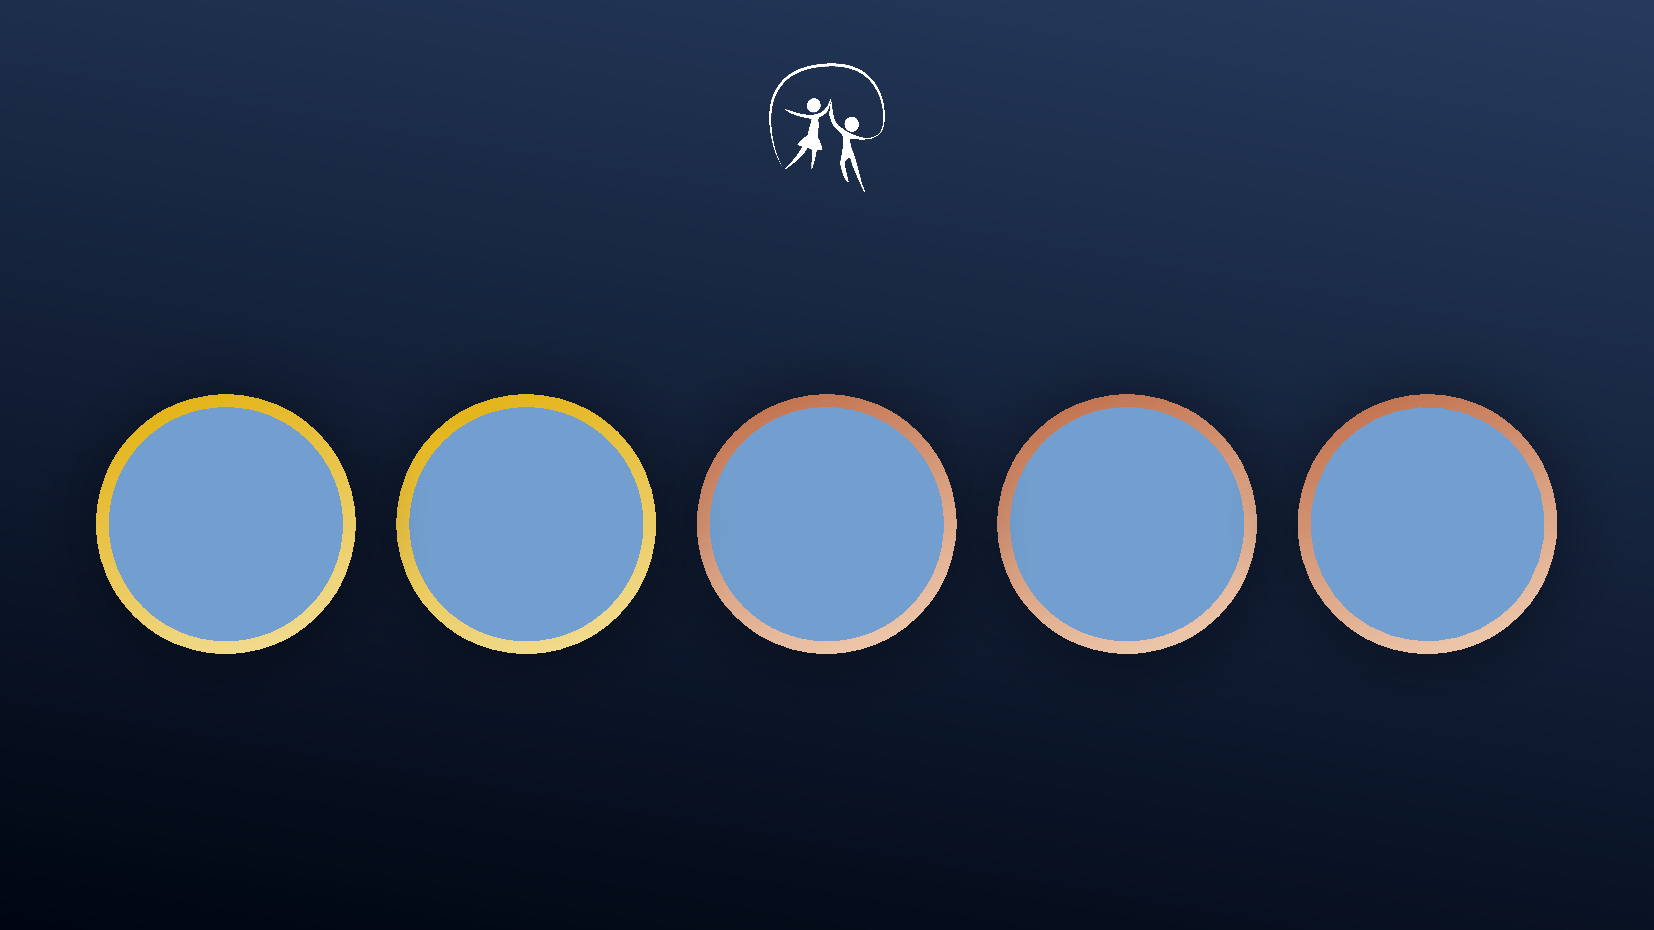
\includegraphics[width=\pdfpagewidth]{images/bg-picture.pdf}}
\setbeamertemplate{navigation symbols}{}


\begin{document}

{
\begin{frame}

% text for the committee
\begin{textblock*}{\pdfpagewidth}(0cm, 2.1cm)
    \centering
    \textbf{\textcolor{white}{\large {{committee}} }}
\end{textblock*}

% text for the subtitle
\begin{textblock*}{\pdfpagewidth}(0cm, 2.9cm)
    \centering
    \textcolor{white}{\normalsize Ισότητα δικαιωμάτων ανδρών και γυναικών}
\end{textblock*}

\begin{tikzpicture}[remember picture, overlay]
    % intentionally commented; creates grid for placing the images absolutely
    % \foreach \x in {0,...,12} \path (current page.south west) +(\x,0.25) node {\small$\x$};
    % \foreach \y in {0,...,9} \path (current page.south west) +(0.25,\y) node {\small$\y$};
    % \foreach \x in {0,0.5,...,12.5} \draw (current page.south west) ++(\x,0) -- +(0,9.6);
    % \foreach \y in {0,0.5,...,9.5} \draw (current page.south west) ++(0,\y) -- +(12.8,0);

    % the pictures of the 5 winners 
    \draw (current page.south west) +(0.93, 3.2) node[anchor=south west] {\includegraphics[width=2.28cm]{images/{{image0}}}};
    \draw (current page.south west) +(3.87, 3.2) node[anchor=south west] {\includegraphics[width=2.28cm]{images/{{image1}}}};
    \draw (current page.south west) +(6.81, 3.2) node[anchor=south west] {\includegraphics[width=2.28cm]{images/{{image2}}}};
    \draw (current page.south west) +(9.75, 3.2) node[anchor=south west] {\includegraphics[width=2.28cm]{images/{{image3}}}};
    \draw (current page.south west) +(12.68, 3.2) node[anchor=south west] {\includegraphics[width=2.28cm]{images/{{image4}}}};

\end{tikzpicture}

% The text below each of the 5 pictures from left to right
% 0
% prize 0
\begin{textblock*}{3cm}(0.675cm, 6.65cm)
    \centering
    \textcolor{white}{\tiny \bf{{award0}} \\}
\end{textblock*}

% name 0
\begin{textblock*}{3cm}(0.675cm, 7.5cm)
    \centering
    \textcolor{white}{\scriptsize {{surname0}} {{name0}} \\}
\end{textblock*}

% country 0
\begin{textblock*}{3cm}(0.675cm, 8.4cm)
    \centering
    \textcolor{white}{\tiny \it {{country0}} \\}
\end{textblock*}

% 1
% prize 1
\begin{textblock*}{2.95cm}(3.65cm, 6.65cm)
    \centering
    \textcolor{white}{\tiny \bf{{award1}} \\}
\end{textblock*}

% name 2
\begin{textblock*}{2.95cm}(3.65cm, 7.5cm)
    \centering
    \textcolor{white}{\scriptsize {{surname1}} {{name1}} \\}
\end{textblock*}

% country 1
\begin{textblock*}{2.95cm}(3.65cm, 8.4cm)
    \centering
    \textcolor{white}{\tiny \it {{country1}} \\}
\end{textblock*}

% 2
% prize 2
\begin{textblock*}{2.95cm}(6.6cm, 6.65cm)
    \centering
    \textcolor{white}{\tiny \bf{{award2}}\\}
\end{textblock*}

% name 2
\begin{textblock*}{2.95cm}(6.6cm, 7.5cm)
    \centering
    \textcolor{white}{\scriptsize {{surname2}} {{name2}} \\}
\end{textblock*}

% country 2
\begin{textblock*}{2.95cm}(6.6cm, 8.4cm)
    \centering
    \textcolor{white}{\tiny \it {{country2}} \\}
\end{textblock*}

% 3
% prize 3
\begin{textblock*}{2.95cm}(9.55cm, 6.65cm)
    \centering
    \textcolor{white}{\tiny \bf{{award3}}\\}
\end{textblock*}

% name 3
\begin{textblock*}{2.95cm}(9.55cm, 7.5cm)
    \centering
    \textcolor{white}{\scriptsize {{surname3}} {{name3}} \\}
\end{textblock*}

% country 3
\begin{textblock*}{2.95cm}(9.55cm, 8.4cm)
    \centering
    \textcolor{white}{\tiny \it {{country3}} \\}
\end{textblock*}

% 4
% prize 4
\begin{textblock*}{2.95cm}(12.5cm, 6.65cm)
    \centering
    \textcolor{white}{\tiny \bf{{award4}}\\}
\end{textblock*}

% name 4
\begin{textblock*}{2.95cm}(12.5cm, 7.5cm)
    \centering
    \textcolor{white}{\scriptsize {{surname4}} {{name4}} \\}
\end{textblock*}

% country 4
\begin{textblock*}{2.95cm}(12.5cm, 8.4cm)
    \centering
    \textcolor{white}{\tiny \it {{country4}} \\}
\end{textblock*}

\end{frame}
}


\end{document}
